\documentclass[../AdvancementSummary.tex]{subfiles}

\begin{document}


%%%%%%%%%%%%%%%%%%%%%%%%%%%%%%%%%%%%%%%%%%%%%%%%%%%
\section{Introduction}
%%%%%%%%%%%%%%%%%%%%%%%%%%%%%%%%%%%%%%%%%%%%%%%%%%%

%
%An individual molecule of a protein with a specific, rigid structure can exhibit complex behavior such as allostery (where modification of one region of the molecule influences a distal region), cooperativity (in which the first few interactions enhance subsequent interactions) and conformational changes. On the other hand, many bio-molecules have floppy, polymer-like geometry with no rigid structure, especially proteins involved in signal transduction \cite{Dyson:2005jb} including in the T Cell Receptor signaling cascade. What properties do floppy molecules endow signaling cascades with? What are their advantages over rigid, structured molecules, which \textit{a priori} appear more tunable? Recent theoretical \cite{Lenz:2006eo} and experimental \cite{Wright:2015cw} work has shown that a floppy polymer that becomes structured upon binding to a ligand, combined with multiple phosphorylation, can exhibit cooperativity.  
%
%One example of an unstructured, floppy molecule is offered by the T Cell Receptor (TCR). While the extra-cellular and intra-membrane regions of TCR are structured, the intra-cellular component, including multiple immuno-tyrosine activation motifs (ITAM) termed the zeta-chain, lacks clear structure and is therefore hypothesized to be floppy. Each human zeta-chain has seven tyrosine phosphorylation sites which are phosphorylated, probably by the kinase Lck, during immunological activation of the T cell. This multiple phosphorylation event comprises a key step in ``kinetic proofreading" \cite{VanDerMerwe:2010hh}, a mechanism that endows the T cell with the exquisite specificity necessary for healthy immune function. 
%
%%%%%%%%%%%%%%%%% 
%\begin{figure}[h!]
%\centering
%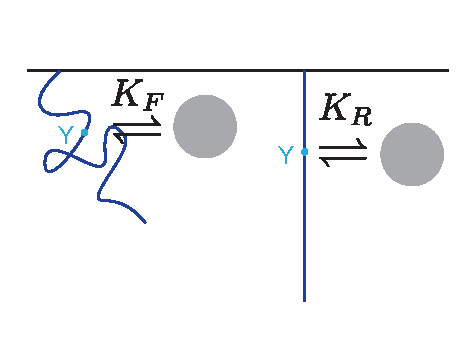
\includegraphics[width=8cm]{figEntropicPenalty.pdf}
%%\caption{ xxxx }
%\label{fig::accuracyFlowchart}
%\end{figure}
%%%%%%%%%%%%%%%%% 
%
%Little is known about the biophysical properties of the zeta-chain (or indeed any unstructured protein domain, which elude crystallography studies). What phosphorylation kinetics are possible? If phosphorylation modifies the polymer properties, e.g., transitions between floppy/unstructured and rigid/structured, can this give rise to cooperativity of phosphorylation and, if so, with what quantitative properties?
%
%
%
%In this project we will perform equilibrium simulations of the zeta-chain interacting with the Lck kinase domain under various assumptions about the effects of phosphorylation. Our aim is to get quantitative estimates and upper bounds for the cooperativity, and other nontrivial kinetics, that can result from the entropic effects of binding to a rigid versus floppy polymer.
%
%
%\textbf{Working title: } Disordered protein domains endow signaling cascades with inherently cooperative kinetics. \textbf{Major question:} What are the ``design advantages" of disordered, polymer domains in signaling? \textbf{Specific question:} What are the cooperativity properties of a multiply-phosphorylated, disordered (floppy) protein that becomes structured (rigid) upon phosphorylation? How does this apply to the T cell signaling cascade, including phosphorylation of the T Cell Receptor zeta-chain by the protein tyrosine kinase Lck? Can this mechanism give rise to high-Hill-number (i.e., ultrasensitive) cooperativity or other nontrivial kinetics? \textbf{Here we: } perform equilibrium calculations of a floppy polymer interacting with a kinase domain under various assumptions about how phosphorylation influences the polymer's structure. We specifically apply results to the TCR zeta-chain and obtain an upper bound on cooperativity in this system. 


%%%%%%%%%%%%%%%%%%%%%%%%%%%%%%%%%%%%%%%%%%%%%%%%%%%
%\section*{Some reading}
%%%%%%%%%%%%%%%%%%%%%%%%%%%%%%%%%%%%%%%%%%%%%%%%%%%
%
%Papers marked with $^{\bullet}$ are of notable interest.
%
%\begin{itemize} 
%\item Background physical chemistry: \citet{Boal:jgXY0Y5Y} \S 3$^{\bullet}$, \citet{Bressloff:RE98Gs4d} \S 1 (free at UCI online)
%\item Reviews: \citet{Wright:2015cw}, \citet{VanDerMerwe:2010hh}, \citet{Brownlie:2013kz}
%\item Primarily theory research papers: \citet{Lenz:2006eo}$^{\bullet}$, \citet{Pontius:1993vu}, \citet{Allard:2012gy}
%\end{itemize}

%%%%%%%%%%%%%%%%%%%%%%%%%%%%%%%%%%%%%%%%%%%%%%%%%%%

Traditionally, studies of protein function have gone hand-in-hand with studies of protein structure. Proteins such as hemoglobin exhibit complicated behavior, such as cooperativity, through modification of their structure. The cooperative transition of hemoglobin from a `tense' to `relaxed' state is well studied with the aid of crystallography and other structure elucidation tools \cite{Jensen1998}.

Of more recent interest are intrinsically disordered proteins (IDPs). These proteins lack a defined structure and are capable of assuming many different conformations. Although examples of IDPs have been reported since the 1970s, it was only in the past two decades that they became a focus of major research \cite{Dunker2008}. 

%As our understanding of disordered proteins develops, so too will our understanding of a variety of cellular behaviors. These studies will elucidate aspects of signaling, cytoskeleton formation, and clustered reactions. Investigations into how disordered proteins mediate each of these processes may lead to new drug targets or introduce new directions for synthetic biology.

Studies have shown that disordered proteins or disordered domains are present in at least 40\% of human proteins, including those involved with signal propagation \cite{Tompa2012}. General functions of IDPs include as tethers between two globular domains \cite{Gonfloni1997}, receptor subunits in signaling pathways \cite{Duchardt2007}, tethers to the membrane \cite{Keir2008}, and facilitators to actin polymerization \cite{Kovar2004, Romero2004}. Given the ubiquitous nature of IDPs, many questions arise: How does their existence influence cellular functions such as biochemical reactions, signaling networks, or cytoskeletal structure?  Are there any functions unique to disordered proteins? Can IDPs exhibit the same complicated behavior as structured proteins?

One example of an intrinsically disordered protein is the CD3 $\zeta$ chain, one of six disordered chains composing the T Cell Receptor (TCR) intracellular region. This molecule facilitates signal propagation in the TCR network in the immune system. An antigen binding to the extracellular regions of the TCR creates a signal transmitted via a chain of events into the cell to the intracellular components of the TCR including the CD3$\zeta$ chain. CD3$\zeta$ undergoes multiple phosphorylation by kinase Lck before another molecule, ZAP-70 can attach and propagate the signal downstream. Ultimately, TCR stimulation by an antigen can result in T cell activation, characterized by events such as proliferation, differentiation, cytoskeletal reorganization, cytotoxicity and cytokine production \cite{Smith-Garvin2009, Lever2016}.

%CELLSignal.com for citation?

We have already demonstrated that disordered proteins can lead to nonlinear signaling behavior. Experiments with only a reconstituted mouse CD3$\zeta$ dimer, simplified extracellular receptor, kinase, and phosphatase reveal that the number of tyrosines impacts the potency and maximum phosphorylation but not the switch-like response \cite{Mukhopadhyay2016}. Our initial differential equation models indicate that to achieve these characteristics, there would need to be a phosphorylation-dependent enhancement of more than 100-fold. That is, the sixth phosphorylation event would be at least 100-fold faster than the first phosphorylation event \cite{Mukhopadhyay2016}. 

\begin{figure}
	\begin{center}
		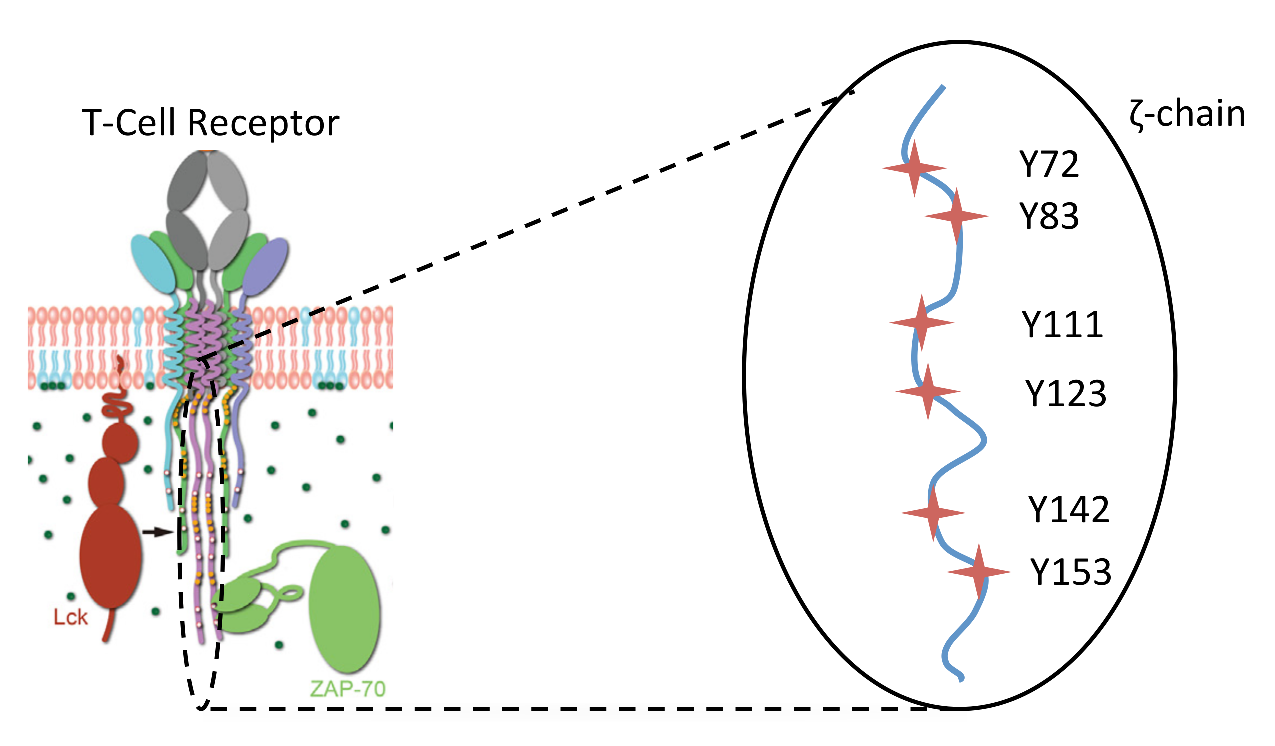
\includegraphics[width=0.8\linewidth]{Figures/TCRDiagram.eps}
	\end{center}
\caption{Cartoon of T Cell Receptor network (left) from \cite{Wu2015}. Location of tyrosines in single $\zeta$ chain (right). \label{fig: TCRCartoon}}
\end{figure}


%%%%%%%%%%%%%%%%%%%%%%%%%%%%%%%%%%%%%%%%%%%%%%%%%%%%
%\subsection{Multisite Phosphorylation}
%%%%%%%%%%%%%%%%%%%%%%%%%%%%%%%%%%%%%%%%%%%%%%%%%%%%
%
%\hl{Stuff about switch-like responses}
%
%Multisite phosphorylation specifically is a well-studied post-translational modification. This phenomenon occurs on both structured and unstructured proteins in many cell systems. \hl{CITE CITE CITE} In signaling pathways, multisite phosphorylation can create ultrasensitivity. \hl{Dushek et al Biophys J 2011 - read} \hl{cite, anything else?} Ultrasensitivity creates a strong response from small changes in intermediate signals and minimal \hl{none?} response from low signals which reduces the impact of noise. \hl{CD3$\zeta$ - does give ultrasensitivity and we know it or it doesn't and we know it or we don't know?} We want to explore if and how multisite phosphorylation of disordered proteins conveys similar signaling functions.

To explore how IDPs can give rise to this nonlinear signaling behavior, we develop a `mesoscale' model of a disordered protein. Previous work has shown that disordered proteins can be represented with models from polymer physics \cite{VanValen2009, Reeves2011}. The distribution of end-to-end distances for disordered domains matches a worm-like chain (WLC) model with persistence length 3.04\AA \cite{Zhou2001}. Models of disordered proteins using freely-jointed chain (FJC) and WLC converge, with the persistence length for the WLC as half the Kuhn length used for the FJC \cite{VanValen2009}.

%\hl{This suggests $l_k$ = 0.6nm....which is not what we use...not sure how to explain that one. Basically we use the lower limit of what is reasonable and could see what difference it makes either by comparing to N=1/2Nmax or by resimulating.}\hl{Find $l_k$ ~ 0.5 in Mukhopadhyay2016 too}

Alternative models for multisite phosphorylation of IDPs include molecular dynamic, ordinary differential equations, or particle based models. However, FJC or other `mesoscale' approaches reach timescales on the order of microseconds to seconds, which are computationally out of reach for traditional atomic scale MD. This approach also allows us to capture the steric effects of a disordered chain, which are missed by coarser models. 

Representations of disordered proteins as freely-jointed chains have already been used to elucidate properties of IDPs. For instance, the length of tethers between domains controls the effective concentration of one domain seen by the other, such as auto-inhibition of WASP \cite{VanValen2009}. In a second example, the disordered molecule, formin, captures profilin-actin monomers and delivers them to the growing end of actin, increasing the actin polymerization rate. In experimental studies of formin, exerting force on the distal end of formin counterintuitively enhances the polymerization rate two-fold over relaxed formins \cite{Jegou2013}. From our previous work, models of formin as a freely-jointed chain offer an explanation for this phenomenon. A force exerted on a freely-jointed chain extends the polymer, increasing capture of profilin-actin by increasing the availabiltiy of binding sites. This increase of capture rate balances the reduction in delivery rate to have a net positive impact on the actin polymerization rate under some circumstances \cite{Bryant2017}. 


%%
%Since IDPs lack a consistent, rigid structure, they must fluctuate between multiple conformations. If we assume IDPs have no structure at all, then the protein may be in any conformation at any time and in fact would sample all of these conformations. This high degree of structure variability makes ligand binding to a specific binding site more challenging since it is now possible for the protein to transiently block its own binding site. That is, there will be conformations where the region around the binding site is occupied by other segments of the protein, preventing a ligand from occupying that space. In order to explore if and how disordered proteins can provide complex signaling behavior to a network, we create a model of a simple disordered protein using principles from polymer physics.
%
%
%\hl{I feel like I need more here.}
%Using a `mesoscale' modeling approach, we study the role disordered proteins play in signaling networks. We investigate how disordered proteins can convey nonlinear signals to a network and how their characteristics influence this signal. 

%bio premise
Given the above evidence that disordered proteins can give rise to nonlinear signaling behavior, the biological premise of the following projects is that disordered polymer properties alone can create these effects, for example through steric interactions with rigid ligands. 
% modeling premise
The modeling premise is that since disordered proteins take on a wide ensemble of conformations, modeling approaches which focus on structure alone are insufficient. On the other hand, a `mesoscale' modeling approach able to describe conformational ensembles will be able capture the nonlinear signaling properties arising from disorder.

%%%%%%%%%%%%%%%%%%%%%%%%%%%%%%%%%%%%%%%%%%%%%%%%%%%
\end{document}
%%%%%%%%%%%%%%%%%%%%%%%%%%%%%%%%%%%%%%%%%%%%%%%%%%%





